\chapter{Introducción}
El presente Trabajo de Fin de Máster (TFM) se ocupa de resolver una problemática real dentro del campo de la identificación humana \cite{thompson_forensic_2006}. En concreto, se hace uso de métodos de aprendizaje profundo y visión por computador para automatizar una técnica de antropología forense empleada en tareas de estimación del perfil biológico, más específicamente, la estimación de la edad de personas fallecidas a partir de restos óseos. 

Este capítulo introductorio se centra en presentar el problema en detalle, la motivación que nos lleva a enfrentarnos a él y el objetivo principal abordado en este TFM. 


\section{Definición del Problema}
\label{daIntro_ProblemDef}
%Que es la antropología forense
La antropología forense (AF) es la disciplina que se dedica al estudio y análisis detallado de las estructuras óseas del cuerpo humano con propósitos médico-legales \cite{byers_introduction_2016,RefWorks:RefID:17-christensen2019forensic}. Este campo combina conocimientos de la antropología física y de otras ramas afines para proporcionar información clave en investigaciones legales.

La antropología física, a su vez, es el campo que estudia la evolución de la especie humana, así como de las condiciones de vida y salud de distintas poblaciones, tanto antiguas como contemporáneas, mediante estudios osteológicos (del hueso) y somatológicos (del cuerpo) \cite{jurmain_introduction_2018}. Este conocimiento no solo permite un análisis detallado de los restos óseos, sino que también incluye una comprensión integral de los aspectos sociales, culturales y de comportamiento humano \cite{antrofisica}. Los expertos en AF, a través de este enfoque multidisciplinario, examinan minuciosamente los restos óseos para extraer la mayor cantidad posible de información relevante, la cual se utiliza para lograr los siguientes objetivos:

\begin{enumerate}
    \item Establecer la ascendencia y las características morfológicas del fallecido.
    \item Identificar las circunstancias y el modo en que ocurrió la muerte de la persona.
    \item Determinar el tiempo transcurrido desde el fallecimiento.
    \item Colaborar en la recuperación de restos, tanto superficiales como enterrados, que sean de interés para la investigación forense.
    \item Proporcionar información útil para la identificación de personas fallecidas, basándose en las características morfológicas presentes en los huesos humanos.
    \item Analizar el esqueleto de personas vivas con fines médico-legales, como en el caso de la identificación de migrantes o menores desaparecidos.
\end{enumerate}

La estimación del perfil biológico (PB) constituye una de las áreas fundamentales de la AF, e incluye la determinación de la edad, el sexo, la estatura y el origen poblacional o ascendencia, además de cualquier otra particularidad que ayude a individualizar los restos, ya sea total o parcialmente esqueletizados. La finalidad de esta evaluación es facilitar la búsqueda de la identidad de una persona desaparecida y, de ser posible, lograr una identificación positiva y certera. Un esquema ilustrativo del proceso de identificación forense puede apreciarse en la Figura \ref{fig:intro_1}.

\begin{figure}[h]
    \centering
    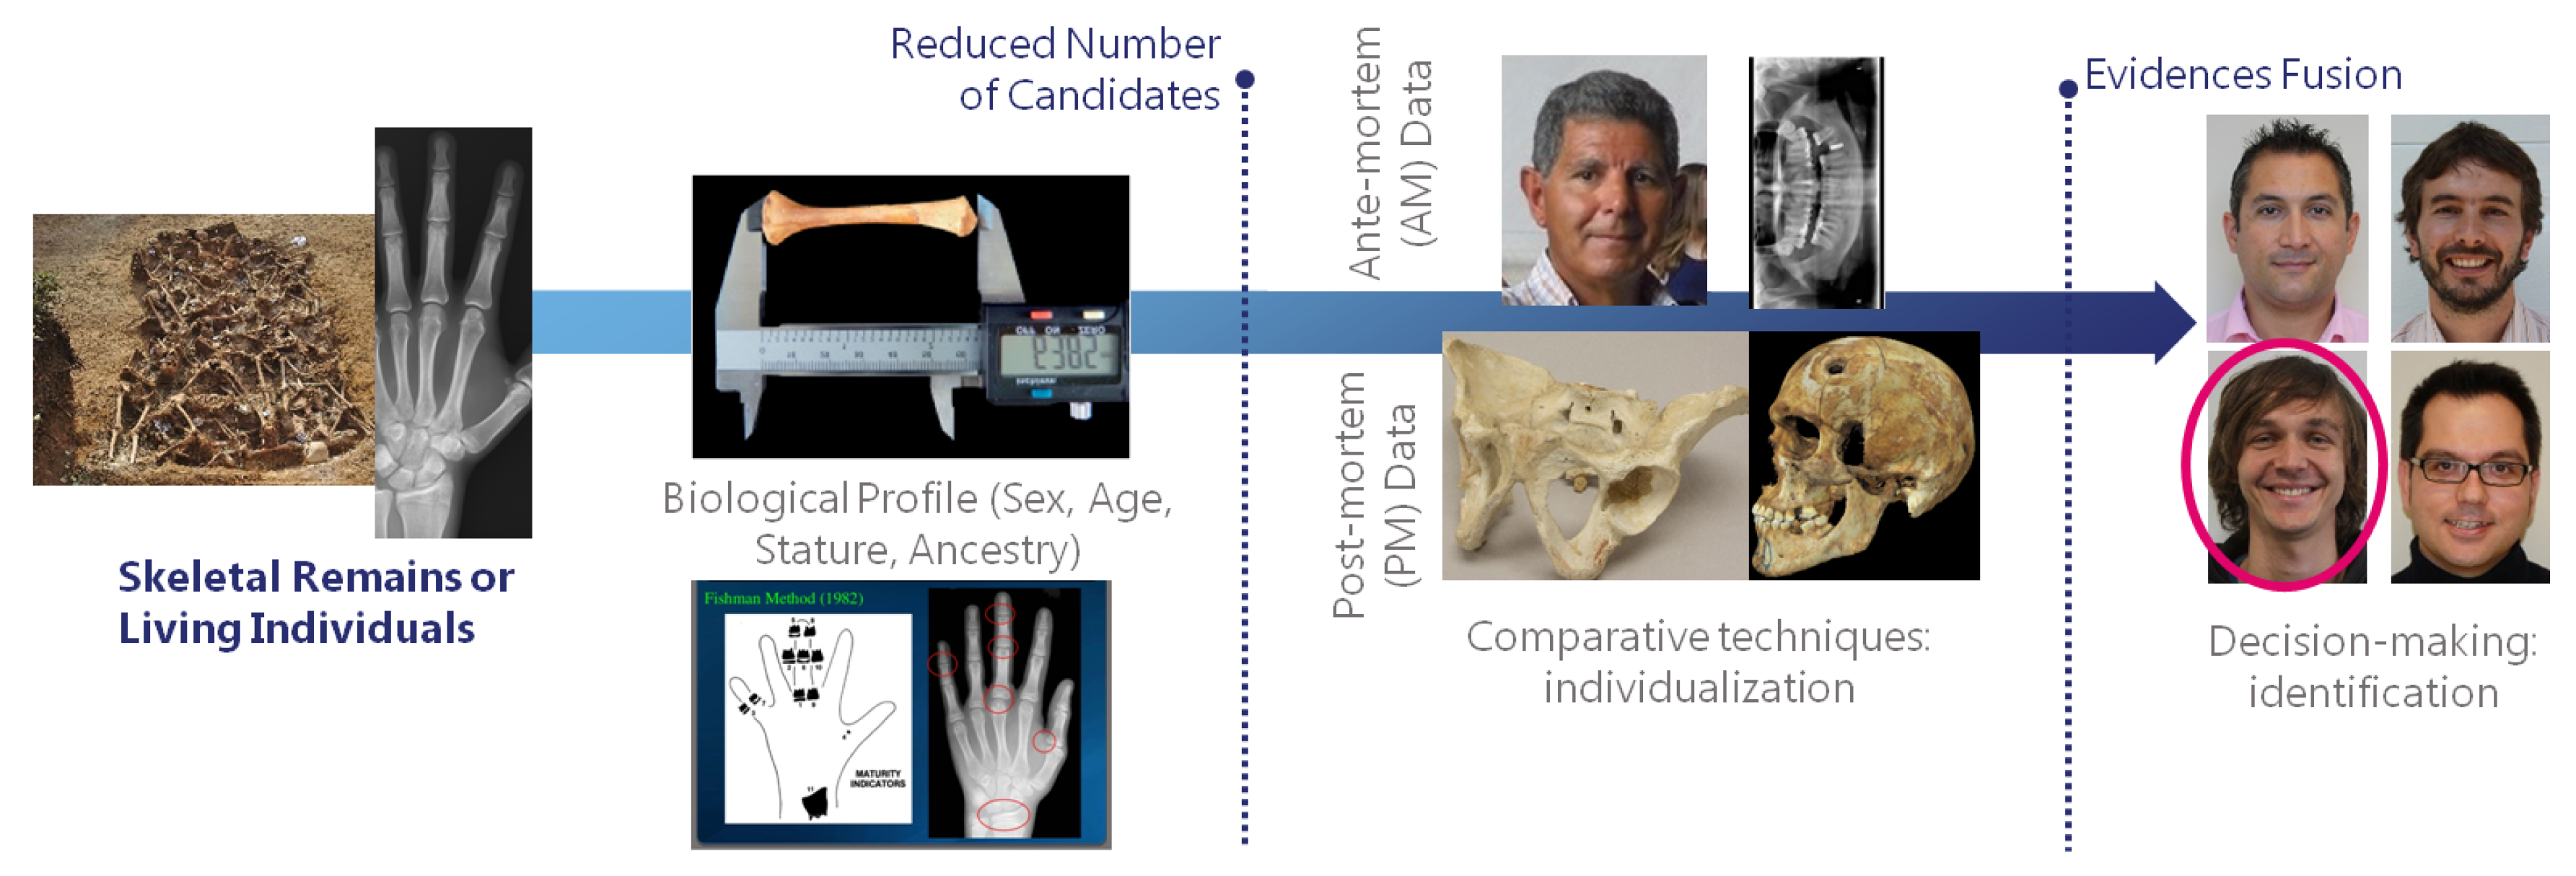
\includegraphics[width=1\linewidth]{figures/1_introduction/intro_1.png}
    \caption[Proceso de identificación forense a partir de restos óseos]{Proceso de identificación forense a partir de restos óseos \cite{RefWorks:RefID:21-mesejo2020survey}.}
    \label{fig:intro_1}
\end{figure}

Uno de los aspectos fundamentales del PB es la estimación de la edad de los restos. Para lograrlo, se examinan estructuras como las suturas craneales \cite{skullAF}, las costillas \cite{icscan1984age}, la cara auricular del ilion \cite{buckberry_age_2002} y la sínfisis del pubis \cite{garvin_current_2012}, estos dos últimos localizados en la pelvis. En cada caso, se observa el grado de desgaste que presentan estos huesos en el momento del fallecimiento, lo cual permite aproximarse a la edad del individuo \cite{RefWorks:RefID:12-black2011forensic}.

La sínfisis del pubis es el hueso más utilizado para estimar la edad de un individuo ya fallecido, siendo la opción preferida por el 95\% de los antropólogos forenses \cite{garvin_current_2012}. El método predominante se fundamenta en el trabajo pionero de Thomas Wingate Todd \cite{RefWorks:RefID:19-todd1921age}, quien en 1921 documentó las transformaciones progresivas de la sínfisis del pubis con el envejecimiento, permitiendo estimar un rango aproximado de edad al momento del fallecimiento. Todd propuso un sistema de etapas de envejecimiento que ha sido revisado y perfeccionado en múltiples ocasiones, siendo la revisión de Suchey-Brooks \cite{RefWorks:RefID:20-brooks1990skeletal}, publicada en 1990, posiblemente la más reconocida de todas. Tanto el método original de Todd como la revisión de Suchey-Brooks se basan en el análisis de diferentes características de la sínfisis del pubis. En función del estado de cada una, asignan atributos categóricos que reflejan el grado de erosión ósea en distintas áreas, permitiendo así calcular un rango estimado de edad para el difunto. Dichas características varían según el método, en este TFM se utilizan las 9 características propuestas por Villar et al. \cite{villar2017first} para el método de Todd, que se detallan en la Tabla \ref{table:themBones}, y en la Tabla \ref{themBomes:visualExample} se presenta un ejemplo visual de cada una de ellas.

\begin{table}[h]
    \centering
% \resizebox{\textwidth}{!}{%
\begin{tabular}{ccc}
    \hline
    \rowcolor[HTML]{D33333} 
    \multicolumn{1}{c|}{\cellcolor[HTML]{D33333}{\color[HTML]{FFFFFF} Característica}} & \multicolumn{2}{c}{\cellcolor[HTML]{D33333}{\color[HTML]{FFFFFF} Etiquetas}} \\ \hline
    \rowcolor[HTML]{FFCCC9} 
    \multicolumn{1}{|c}{\cellcolor[HTML]{FD6864}Crestas y Surcos} & Porosidad Regular & \multicolumn{1}{c|}{\cellcolor[HTML]{FFCCC9}Muy Definidas} \\ \cline{1-1}
    \multicolumn{1}{c|}{} & \cellcolor[HTML]{FFCCC9}Poco Profundas & \multicolumn{1}{c|}{\cellcolor[HTML]{FFCCC9}Restos de Surcos} \\ \cline{3-3} 
    \multicolumn{1}{c|}{} & \multicolumn{1}{c|}{\cellcolor[HTML]{FFCCC9}No hay surcos} &  \\ \hline
    \rowcolor[HTML]{FFCCC9} 
    \multicolumn{1}{|c}{\cellcolor[HTML]{FD6864}Porosidad Irregular} & No & \multicolumn{1}{c|}{\cellcolor[HTML]{FFCCC9}Mediana} \\ \cline{1-1} \cline{3-3} 
    \multicolumn{1}{c|}{} & \multicolumn{1}{c|}{\cellcolor[HTML]{FFCCC9}Si} &  \\ \hline
    \rowcolor[HTML]{FFCCC9} 
    \multicolumn{1}{|c}{\cellcolor[HTML]{FD6864}Borde Superior} & No Definido & \multicolumn{1}{c|}{\cellcolor[HTML]{FFCCC9}Definido} \\ \hline
    \rowcolor[HTML]{FFCCC9} 
    \multicolumn{1}{|c}{\cellcolor[HTML]{FD6864}Nódulo Óseo} & Ausente & \multicolumn{1}{c|}{\cellcolor[HTML]{FFCCC9}Presente} \\ \hline
    \rowcolor[HTML]{FFCCC9} 
    \multicolumn{1}{|c}{\cellcolor[HTML]{FD6864}Borde Inferior} & No Definido & \multicolumn{1}{c|}{\cellcolor[HTML]{FFCCC9}Definido} \\ \hline
    \rowcolor[HTML]{FFCCC9} 
    \multicolumn{1}{|c}{\cellcolor[HTML]{FD6864}Plataforma Dorsal} & Ausente & \multicolumn{1}{c|}{\cellcolor[HTML]{FFCCC9}En Formación} \\ \cline{1-1} \cline{3-3} 
    \multicolumn{1}{l|}{} & \multicolumn{1}{c|}{\cellcolor[HTML]{FFCCC9}Presente} & \multicolumn{1}{l}{} \\ \hline
    \rowcolor[HTML]{FFCCC9} 
    \multicolumn{1}{|c}{\cellcolor[HTML]{FD6864}Borde Dorsal} & Ausente & \multicolumn{1}{c|}{\cellcolor[HTML]{FFCCC9}En Formación} \\ \cline{1-1} \cline{3-3} 
    \multicolumn{1}{l|}{} & \multicolumn{1}{c|}{\cellcolor[HTML]{FFCCC9}Presente} & \multicolumn{1}{l}{} \\ \hline
    \rowcolor[HTML]{FFCCC9} 
    \multicolumn{1}{|c}{\cellcolor[HTML]{FD6864}Bisel Ventral} & Ausente & \multicolumn{1}{c|}{\cellcolor[HTML]{FFCCC9}En Formación} \\ \cline{1-1} \cline{3-3} 
    \multicolumn{1}{c|}{} & \multicolumn{1}{c|}{\cellcolor[HTML]{FFCCC9}Presente} &  \\ \hline
    \rowcolor[HTML]{FFCCC9} 
    \multicolumn{1}{|c}{\cellcolor[HTML]{FD6864}Borde Ventral} & Ausente & \multicolumn{1}{c|}{\cellcolor[HTML]{FFCCC9}En Formación} \\ \cline{1-1}
    \multicolumn{1}{c|}{} & \cellcolor[HTML]{FFCCC9}Formado, Sin Excrecencias & \multicolumn{1}{c|}{\cellcolor[HTML]{FFCCC9}Formado, Pocas Excrecencias} \\ \cline{3-3} 
    \multicolumn{1}{c|}{} & \multicolumn{1}{c|}{\cellcolor[HTML]{FFCCC9}Formado, Muchas Excrecencias} &  \\ \cline{2-2}
\end{tabular}%
% }
\caption[Método de Todd: Características para determinación de edad]{Características utilizadas para la determinación de la edad según el método de Todd \cite{RefWorks:RefID:19-todd1921age} propuestos por Villar et al. \cite{villar2017first}.}
\label{table:themBones}
\end{table}

\begin{table}[h]
\centering
\resizebox{\textwidth}{!}{%
\begin{tabular}{|
    >{\columncolor[HTML]{D33333}}c |c|c|c|c|c|c|c|}
    \hline
    {\color[HTML]{FFFFFF} \textbf{Característica}} & \begin{tabular}[c]{@{}c@{}}Crestas y\\ Surcos\end{tabular} & \begin{tabular}[c]{@{}c@{}}Porosidad\\ Irregular\end{tabular} & \begin{tabular}[c]{@{}c@{}}Borde \\ Superior\end{tabular} & \begin{tabular}[c]{@{}c@{}}Nódulo\\ Óseo\end{tabular} & \begin{tabular}[c]{@{}c@{}}Borde\\ Inferior\end{tabular} & \begin{tabular}[c]{@{}c@{}}Borde\\ Dorsal\end{tabular} & \begin{tabular}[c]{@{}c@{}}Plataforma\\ Dorsal\end{tabular} \\ \hline
    {\color[HTML]{FFFFFF} \textbf{Atributo}} & Muy Definidos & Sí & Definido & Presente & Definido & Definido & Presente \\ \hline
    {\color[HTML]{FFFFFF} \textbf{Ejemplo}} & 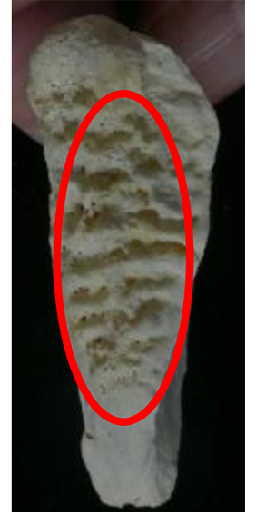
\includegraphics[align=c, width=0.2\linewidth]{figures/1_introduction/todd1.png} & 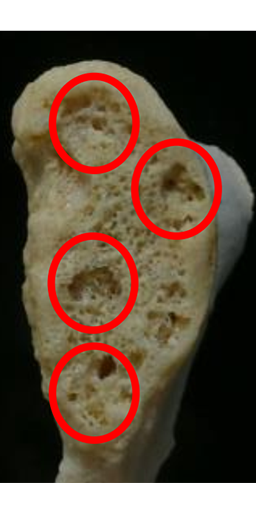
\includegraphics[align=c, width=0.2\linewidth]{figures/1_introduction/todd2.png} & 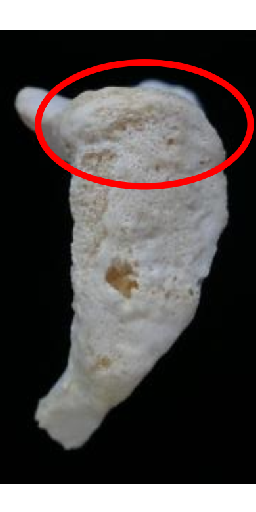
\includegraphics[align=c, width=0.2\linewidth]{figures/1_introduction/todd3.png} & 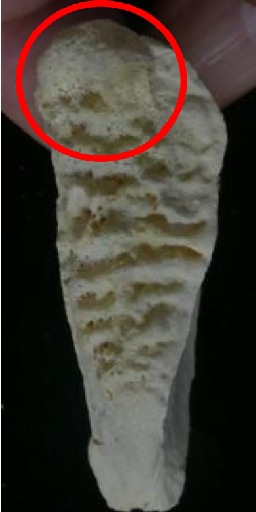
\includegraphics[align=c, width=0.2\linewidth]{figures/1_introduction/todd4.png} & 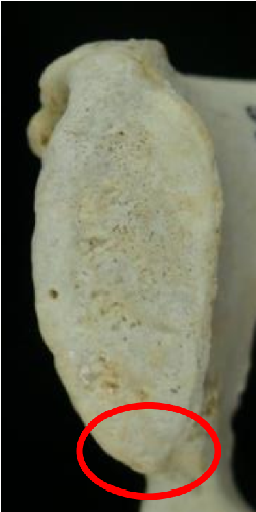
\includegraphics[align=c, width=0.2\linewidth]{figures/1_introduction/todd5.png} & 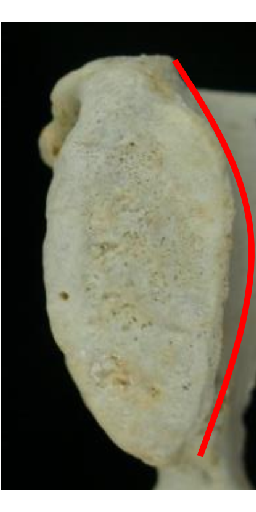
\includegraphics[align=c, width=0.2\linewidth]{figures/1_introduction/todd6.png} & 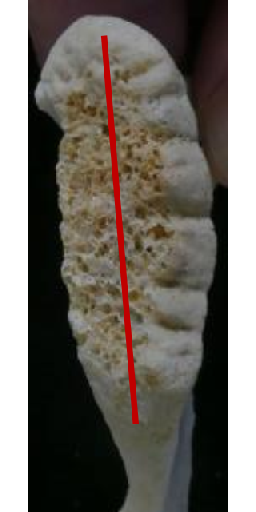
\includegraphics[align=c, width=0.2\linewidth]{figures/1_introduction/todd7.png}   \\ \hline
\end{tabular}%
}
\caption[Método de Todd: Ejemplo de características]{Ejemplo de las características del método de Todd y sus derivados propuestos por Villar et al. \cite{villar2017first}}
\label{themBomes:visualExample}
\end{table}

Es importante destacar que la metodología empleada, al igual que en muchas otras de la AF, depende en gran medida del criterio subjetivo del experto. Esto genera errores intra- e inter-experto \cite{irurita2025pubic}, ya que el uso de criterios subjetivos y descriptivos introduce limitaciones debido a las diversas interpretaciones entre evaluadores \cite{RefWorks:RefID:12-black2011forensic}. Tal situación disminuye la confiabilidad y validez de los resultados obtenidos, lo que finalmente reduce la credibilidad de los estudios forenses cuando se presentan como evidencia en un juicio (como se indicará más abajo cuando se mencione el estándar de Daubert). Esta problemática justifica la búsqueda de herramientas y metodologías que, al menos parcialmente, mitiguen dichas limitaciones. En este contexto, disciplinas como la inteligencia artificial (IA) \cite{russell_artificial_2021} y, en particular, el aprendizaje automático (\textit{Machine Learning}, ML) \cite{abu-mostafa_learning_2012, bishop_pattern_2019, murphy_probabilistic_2022, murphy_probabilistic_2023}, el aprendizaje profundo (\textit{Deep Learning}, DL) \cite{Goodfellow-et-al-2016, bishop_deep_2024, prince_understanding_2023} y la visión por computador (\textit{Computer Vision}, CV) \cite{torralba_foundations_2024, szeliski_computer_2022} pueden asistir, automatizar y acelerar las tareas forenses, reduciendo significativamente los sesgos y errores.

Considerando todo lo anterior, \textbf{el presente TFM se centra en la clasificación automática de las características morfológicas de la sínfisis del pubis para estimar la edad a partir de modelos 3D mediante técnicas de IA.}

\section{Motivación}
En las últimas décadas los avances en IA, especialmente en ML y CV, han facilitado tanto la automatización de tareas repetitivas y tediosas como la superación del rendimiento humano en actividades complejas. En estos ámbitos, se han logrado avances significativos en tareas como la clasificación y segmentación de imágenes \cite{edozie_comprehensive_2025}, la detección de objetos en las mismas \cite{liu_deep_2020}, generación de imagen y vídeo \cite{wang_generative_2021} así como la reconstrucción de imágenes \cite{xie_review_2022}. Estas técnicas han sido ampliamente adoptadas en diversas disciplinas \cite{chai_deep_2021}, incluida la medicina, donde han proporcionado herramientas de gran utilidad para los profesionales del área \cite{esteva_deep_2021}.

No obstante, resulta sorprendente que, en la actualidad, la AF siga presentando un nivel relativamente bajo de sofisticación tecnológica \cite{RefWorks:RefID:21-mesejo2020survey}. En este contexto, una de las principales motivaciones de este trabajo es impulsar la modernización y automatización de la AF desde una perspectiva tecnológica, centrándose particularmente en la aplicación de técnicas avanzadas para la estimación de edad.

Además, como se mencionó previamente, la subjetividad inherente a la AF representa un desafío desde el punto de vista legal. En muchos casos, los análisis carecen de una base científica sólida según el criterio de Daubert \cite{noauthor_daubert_nodate}, el cual establece los requisitos para la admisibilidad del testimonio experto en un juicio. Según este criterio, un método es válido si: (1) los resultados son reproducibles y han sido verificados por terceros, (2) posee tasas de error conocidas y (3) es aceptado por la comunidad científica forense.

En este sentido, la aplicación de IA en AF puede contribuir significativamente a la reducción de la subjetividad en las identificaciones, minimizando errores humanos, y acelerando la realización de múltiples tareas, estructurando el conocimiento experto y facilitando la obtención de nuevos hallazgos. Esto, a su vez, fortalecería la base científica de los métodos utilizados en la disciplina, permitiendo que sean reproducibles y que se conozcan con precisión sus tasas de error, lo que favorecería su cumplimiento con el criterio de Daubert y su aceptación en el ámbito legal.

Si se analiza el contexto global de la identificación humana, se evidencia que la estimación del PB mediante técnicas de AF adquiere especial relevancia, puesto que otras herramientas de mayor precisión y sofisticación, como el análisis de ADN o la toma de huellas dactilares, presentan limitaciones significativas \cite{de_boer_role_2019, beauthier_mass_2009}. Por ejemplo, el análisis de ADN requiere una inversión elevada en recursos y tiempo, y al igual que la obtención de huellas dactilares, depende de la disponibilidad de datos tanto ante-mortem como post-mortem. Además, ambas técnicas se ven afectadas por el estado de los tejidos blandos, que son los más susceptibles a la descomposición natural o a daños provocados por quemaduras y exposición a agua o productos químicos, entre otros factores. En cambio, el tejido óseo, en general, demuestra una mayor resistencia y es frecuentemente lo único recuperable tras la completa descomposición de los tejidos blandos. Por ello, las técnicas basadas en AF son especialmente útiles en los siguientes escenarios:

\begin{itemize}
    \item Identificación masiva de víctimas de desastres naturales, accidentes o ataques terroristas.
    \item Identificación de víctimas de conflictos armados o actos de lesa humanidad, donde los restos pueden estar desmembrados, desfigurados y/o quemados.
    \item Procesamiento de fosas comunes en las que los restos óseos se han mezclado.
    \item Identificación de personas desaparecidas en contextos no relacionados con desastres o guerras, en los que las condiciones del cadáver han impedido la aplicación de otras técnicas \cite{byers_introduction_2016}.
\end{itemize}

Para dimensionar el desafío al que se enfrentan los antropólogos forenses, es relevante considerar que, únicamente en el año 2019, 20,000 personas perdieron la vida por causas vinculadas al terrorismo, con un promedio anual de 24,000 muertes en la última década atribuibles a este fenómeno \cite{owid_terrorism}. Asimismo, los desastres naturales ocasionan aproximadamente entre 40,000 y 50,000 muertes anuales \cite{owid_natural_disasters}. En el caso de Gaza, al momento de la redacción de este documento, se estima que entre 56,000 y 80,000 personas han sido asesinadas como resultado de los bombardeos, mientras que al menos 11.000 permanecen desaparecidas bajo los escombros, según datos del Ministerio de Salud y la ONU \cite{morales_56000_2025}. En España, aún se deben recuperar alrededor de 20,000 víctimas de la Guerra Civil, muchas de las cuales se hallan en fosas y cunetas, de modo que apenas un tercio de ellas podría ser identificada mediante análisis de ADN \cite{junquera_huellas_2022}.

Estos datos subrayan la necesidad de incorporar técnicas informáticas automatizadas en el ámbito de la AF, ya que permitirían una considerable optimización en términos de tiempo y recursos, facilitando la detección de las características determinantes para la estimación de la edad en situaciones en las que el número de individuos a identificar es elevado y otras técnicas no son aplicables.

\section{Objetivos}

Tras haber descrito el problema y su motivación, el objetivo principal de este TFM consiste en desarrollar y validar un modelo de aprendizaje profundo que, a partir de modelos 3D de la sínfisis púbica, permita extraer características morfológicas relevantes para la estimación de la edad en el momento de la muerte.

Cabe destacar que este trabajo se construye como una continuación directa del TFG desarrollado previamente por el propio autor \cite{lugli_tfg_2022}. En dicho trabajo preliminar se exploraron las primeras aproximaciones al uso de técnicas de DL aplicadas a mallas 3D y en particular a la sínfisis del pubis, centrándose principalmente en la viabilidad del procesamiento geométrico de las mallas y, debido a las limitaciones del conjunto de datos y la infraestructura computacional disponibles en ese momento, solo fue posible abordar la predicción de una de las nueve características morfológicas del método de Todd, aunque se obtuvieron resultados prometedores.

El presente TFM amplía sustancialmente dicho enfoque inicial, incorporando técnicas más actuales y sofisticadas de DL para datos 3D, así como procedimientos más sofisticados para la obtención de la arquitectura e hiperparámetros de dichos modelos. Además, se aborda un volumen experimental considerablemente mayor y se incorpora el análisis del efecto de la resolución de las mallas sobre el rendimiento predictivo así como una visión a la interpretabilidad de los modelos obtenidos. Todo ello con el objetivo de avanzar hacia un sistema más robusto, reproducible y explicable para la clasificación automática de las características morfológicas utilizadas en la estimación de la edad en la muerte.

Este objetivo principal se desglosa en los siguientes objetivos parciales:

\begin{enumerate}
    \item Realizar un estudio exhaustivo de la literatura relativa a la estimación de edad a partir de restos óseos y al procesamiento de modelos 3D mediante redes neuronales profundas.
    \item Analizar y discutir los enfoques y modelos existentes, seleccionando de forma razonada los candidatos más prometedores para el problema abordado.
    \item Evaluar el impacto de la reducción de resolución en mallas 3D de la sínfisis del pubis sobre la calidad topológica y la capacidad de predicción del modelo.
    \item Generar, entrenar y evaluar de forma extensiva múltiples arquitecturas de DL con el fin de identificar configuraciones óptimas que permitan predecir con precisión las nueve características morfológicas del método de Todd.
\end{enumerate}

\section{Planificación del proyecto}

%Un TFG consta de 12 créditos ECTS, siendo un crédito igual a 25 horas de trabajo. Se puede calcular que en total se requieren aproximadamente 300 horas totales para la realización del mismo. 

El proyecto presente consiste, en esencia, en el diseño e implementación de un software de investigación. Dicho software posee unos requisitos y objetivos claros, por lo que no se espera que existan grandes cambios en su desarrollo. De cara a planificar el proyecto, resulta fundamental constatar que la asignatura del TFG consta de 12 créditos ECTS, siendo un crédito igual a 25 horas de trabajo. Esto implica que en total, se requieren aproximadamente 300 horas para la realización del mismo. Como el segundo cuatrimestre cuenta con 20 semanas aproximadamente, la realización del TFG requerirá 15 horas semanales (equivalente a 3 horas diarias, 5 días a la semana).

Tomando esto en cuenta, se observa que es un proyecto de complejidad pequeña a mediana respecto a los requisitos y objetivos, por lo que se opta por utilizar la metodología de desarrollo de software en cascada \cite{pressman2005software}. Esta metodología posee las fases de análisis, diseño, codificación, pruebas y mantenimiento. Dicho esto, el modelo en cascada rara vez se utiliza de forma estricta, pues implica el no poder retroceder a una fase anterior, lo que necesita un previo y absoluto conocimiento de los requisitos, la no volatilidad de los mismos y que las etapas subsiguientes no posean errores. Por eso se utiliza el modelo en cascada con retroalimentación, que permite volver a fases anteriores para realizar pequeños ajustes, sea por errores detectados, ambigüedades, o bien porque los propios requisitos hayan cambiado.

Las fases del ciclo de vida se adaptaron al proyecto de la siguiente forma:
\begin{itemize}
    \item Análisis de Requisitos: Consistió en las reuniones iniciales con el cliente, que en este caso, serían los directores del TFG junto con los antropólogos forenses. Se realiza también en esta fase una revisión bibliográfica extensa en el ámbito de la AF como la combinación de AF con técnicas automáticas dentro del área de la IA con la finalidad de establecer los objetivos del trabajo.
    \item Diseño: Consistió en la investigación y selección de las técnicas aplicables al problema, lo que incluye modelos, métricas, datos y protocolo de validación experimental. Aquí también se incluyen las diversas pruebas preliminares de los modelos.
    \item Implementación: Consintió en la adaptación del código de los modelos investigados, implementación de funcionalidades, así como la implementación de software de soporte en forma de scripts, tanto para la generación, el preprocesado de datos y obtención de diferentes métricas o estadísticas.
    \item Pruebas: Consiste mayoritariamente en la realización de diversos experimentos con los modelos y datos seleccionados.
\end{itemize}
Dicho esto, se puede observar la planificación inicial del proyecto en la Tabla \ref{table:plan1}, donde se mantuvo un mes adicional para posibles imprevistos o retrasos.

\begin{table}[h]
\centering
\resizebox{\textwidth}{!}{%
\begin{tabular}{|c|c|ll|llll|llll|lllll|llll|llll|}
\hline
\rowcolor[HTML]{FFC702} 
\cellcolor[HTML]{FFC702} & \cellcolor[HTML]{FFC702} & \multicolumn{2}{c|}{\cellcolor[HTML]{FFC702}\textbf{Febrero}} & \multicolumn{4}{c|}{\cellcolor[HTML]{FFC702}\textbf{Marzo}} & \multicolumn{4}{c|}{\cellcolor[HTML]{FFC702}\textbf{Abril}} & \multicolumn{5}{c|}{\cellcolor[HTML]{FFC702}\textbf{Mayo}} & \multicolumn{4}{c|}{\cellcolor[HTML]{FFC702}\textbf{Junio}} & \multicolumn{4}{c|}{\cellcolor[HTML]{FFC702}\textbf{Julio}} \\ \cline{3-25} 
\rowcolor[HTML]{FFC702} 
\multirow{-2}{*}{\cellcolor[HTML]{FFC702}\textbf{Tarea}} & \multirow{-2}{*}{\cellcolor[HTML]{FFC702}\begin{tabular}[c]{@{}c@{}}\textbf{Semanas -}\\ \textbf{Horas}\end{tabular}} & \multicolumn{1}{c}{\cellcolor[HTML]{FFC702}21} & \multicolumn{1}{c|}{\cellcolor[HTML]{FFC702}28} & \multicolumn{1}{c}{\cellcolor[HTML]{FFC702}07} & \multicolumn{1}{c}{\cellcolor[HTML]{FFC702}14} & \multicolumn{1}{c}{\cellcolor[HTML]{FFC702}21} & \multicolumn{1}{c|}{\cellcolor[HTML]{FFC702}28} & \multicolumn{1}{c}{\cellcolor[HTML]{FFC702}04} & \multicolumn{1}{c}{\cellcolor[HTML]{FFC702}11} & \multicolumn{1}{c}{\cellcolor[HTML]{FFC702}18} & \multicolumn{1}{c|}{\cellcolor[HTML]{FFC702}25} & \multicolumn{1}{c}{\cellcolor[HTML]{FFC702}02} & \multicolumn{1}{c}{\cellcolor[HTML]{FFC702}09} & \multicolumn{1}{c}{\cellcolor[HTML]{FFC702}16} & \multicolumn{1}{c}{\cellcolor[HTML]{FFC702}23} & \multicolumn{1}{c|}{\cellcolor[HTML]{FFC702}30} & \multicolumn{1}{c}{\cellcolor[HTML]{FFC702}06} & \multicolumn{1}{c}{\cellcolor[HTML]{FFC702}13} & \multicolumn{1}{c}{\cellcolor[HTML]{FFC702}20} & \multicolumn{1}{c|}{\cellcolor[HTML]{FFC702}27} & \multicolumn{1}{c}{\cellcolor[HTML]{FFC702}04} & \multicolumn{1}{c}{\cellcolor[HTML]{FFC702}11} & \multicolumn{1}{c}{\cellcolor[HTML]{FFC702}18} & \multicolumn{1}{c|}{\cellcolor[HTML]{FFC702}25} \\ \hline
Análisis de Requisitos & 4 - 60 & \cellcolor[HTML]{9B9B9B} & \cellcolor[HTML]{9B9B9B} & \cellcolor[HTML]{9B9B9B} & \cellcolor[HTML]{9B9B9B} &  &  &  &  &  &  &  &  &  &  &  &  &  &  &  &  &  &  &  \\ \cline{1-1}
Diseño & 4 - 60 &  &  &  &  & \cellcolor[HTML]{9B9B9B} & \cellcolor[HTML]{9B9B9B} & \cellcolor[HTML]{9B9B9B} & \cellcolor[HTML]{9B9B9B} &  &  &  &  &  &  &  &  &  &  &  &  &  &  &  \\ \cline{1-1}
Implementación & 6 - 90 &  &  &  &  &  &  &  &  & \cellcolor[HTML]{9B9B9B} & \cellcolor[HTML]{9B9B9B} & \cellcolor[HTML]{9B9B9B} & \cellcolor[HTML]{9B9B9B} & \cellcolor[HTML]{9B9B9B} & \cellcolor[HTML]{9B9B9B} &  &  &  &  &  &  &  &  &  \\ \cline{1-1}
Pruebas & 6 - 90 &  &  &  &  &  &  &  &  &  &  &  &  &  &  & \cellcolor[HTML]{9B9B9B} & \cellcolor[HTML]{9B9B9B} & \cellcolor[HTML]{9B9B9B} & \cellcolor[HTML]{9B9B9B} & \cellcolor[HTML]{9B9B9B} & \cellcolor[HTML]{9B9B9B} &  &  &  \\ \hline
\end{tabular}%
}
\caption{Planificación temporal inicial del proyecto}
\label{table:plan1}
\end{table}

Se realizó la planificación inicial con plazos relajados, tomando en cuenta que el autor estaba también realizando las Prácticas de Empresa, junto con estar cursando tres asignaturas. Aún así, ocurrieron retrasos significativos. Una causa fue el método seleccionado ya que, por una parte, es un método muy reciente por lo que la documentación del mismo es escasa y también porque el método utiliza librerías anteriormente desconocidas por el autor, lo que implicó más tiempo del planificado para estudiar y comprender su funcionamiento. Otra causa fueron los datos, pues ocurrió un retraso significativo en la obtención de los mismos, así como tiempo adicional que se utilizó para preprocesarlos, pues por diversas razones esto no se pudo automatizar completamente. Todo ello conllevó una modificación de la planificación, que puede observarse en la Tabla \ref{table:plan2}.

\begin{table}[h]
\resizebox{\textwidth}{!}{%
\begin{tabular}{|c|c|ll|llll|llll|lllll|llll|llll|}
\hline
\rowcolor[HTML]{FFC702} 
\cellcolor[HTML]{FFC702} & \cellcolor[HTML]{FFC702} & \multicolumn{2}{c|}{\cellcolor[HTML]{FFC702}\textbf{Febrero}} & \multicolumn{4}{c|}{\cellcolor[HTML]{FFC702}\textbf{Marzo}} & \multicolumn{4}{c|}{\cellcolor[HTML]{FFC702}\textbf{Abril}} & \multicolumn{5}{c|}{\cellcolor[HTML]{FFC702}\textbf{Mayo}} & \multicolumn{4}{c|}{\cellcolor[HTML]{FFC702}\textbf{Junio}} & \multicolumn{4}{c|}{\cellcolor[HTML]{FFC702}\textbf{Julio}} \\ \cline{3-25} 
\rowcolor[HTML]{FFC702} 
\multirow{-2}{*}{\cellcolor[HTML]{FFC702}\textbf{Tarea}} & \multirow{-2}{*}{\cellcolor[HTML]{FFC702}\begin{tabular}[c]{@{}c@{}}\textbf{Semanas -}\\ \textbf{Horas}\end{tabular}} & \multicolumn{1}{c}{\cellcolor[HTML]{FFC702}21} & \multicolumn{1}{c|}{\cellcolor[HTML]{FFC702}28} & \multicolumn{1}{c}{\cellcolor[HTML]{FFC702}07} & \multicolumn{1}{c}{\cellcolor[HTML]{FFC702}14} & \multicolumn{1}{c}{\cellcolor[HTML]{FFC702}21} & \multicolumn{1}{c|}{\cellcolor[HTML]{FFC702}28} & \multicolumn{1}{c}{\cellcolor[HTML]{FFC702}04} & \multicolumn{1}{c}{\cellcolor[HTML]{FFC702}11} & \multicolumn{1}{c}{\cellcolor[HTML]{FFC702}18} & \multicolumn{1}{c|}{\cellcolor[HTML]{FFC702}25} & \multicolumn{1}{c}{\cellcolor[HTML]{FFC702}02} & \multicolumn{1}{c}{\cellcolor[HTML]{FFC702}09} & \multicolumn{1}{c}{\cellcolor[HTML]{FFC702}16} & \multicolumn{1}{c}{\cellcolor[HTML]{FFC702}23} & \multicolumn{1}{c|}{\cellcolor[HTML]{FFC702}30} & \multicolumn{1}{c}{\cellcolor[HTML]{FFC702}06} & \multicolumn{1}{c}{\cellcolor[HTML]{FFC702}13} & \multicolumn{1}{c}{\cellcolor[HTML]{FFC702}20} & \multicolumn{1}{c|}{\cellcolor[HTML]{FFC702}27} & \multicolumn{1}{c}{\cellcolor[HTML]{FFC702}04} & \multicolumn{1}{c}{\cellcolor[HTML]{FFC702}11} & \multicolumn{1}{c}{\cellcolor[HTML]{FFC702}18} & \multicolumn{1}{c|}{\cellcolor[HTML]{FFC702}25} \\ \hline
Análisis de Requisitos & 5 - 75 & \cellcolor[HTML]{9B9B9B} & \cellcolor[HTML]{9B9B9B} & \cellcolor[HTML]{9B9B9B} & \cellcolor[HTML]{9B9B9B} & \cellcolor[HTML]{9B9B9B} &  &  &  &  &  &  &  &  &  &  &  &  &  &  &  &  &  &  \\ \cline{1-1}
Diseño & 4 - 60 &  &  &  &  &  & \cellcolor[HTML]{9B9B9B} & \cellcolor[HTML]{9B9B9B} & \cellcolor[HTML]{9B9B9B} & \cellcolor[HTML]{9B9B9B} &  &  &  &  &  &  &  &  &  &  &  &  &  &  \\ \cline{1-1}
Implementación & 8 - 120 &  &  &  &  &  &  &  &  &  & \cellcolor[HTML]{9B9B9B} & \cellcolor[HTML]{9B9B9B} & \cellcolor[HTML]{9B9B9B} & \cellcolor[HTML]{9B9B9B} &  &  &  & \cellcolor[HTML]{9B9B9B} & \cellcolor[HTML]{9B9B9B} & \cellcolor[HTML]{9B9B9B} & \cellcolor[HTML]{9B9B9B} &  &  &  \\ \cline{1-1}
Pruebas & 5 - 75 &  &  &  &  &  &  &  &  &  &  &  &  &  & \cellcolor[HTML]{9B9B9B} & \cellcolor[HTML]{9B9B9B} & \cellcolor[HTML]{9B9B9B} &  &  &  &  & \cellcolor[HTML]{9B9B9B} & \cellcolor[HTML]{9B9B9B} &  \\ \hline
\end{tabular}%
}
\caption{Planificación temporal final del proyecto}
\label{table:plan2}
\end{table}

Para el coste estimado, se asume un salario de 35\officialeuro/hora para un responsable I+D de una empresa tecnológica o un investigador senior. Se añade también el costo de los materiales, de los que resalta: el coste del portátil utilizado para el desarrollo del TFG, el coste de dispositivos de almacenamiento masivo, el costo de usar un servidor GPU de altas prestaciones, y el coste acumulado de una suscripción a Google Colab Pro por la duración del proyecto, junto a otros gastos misceláneos. Se puede observar el desglose de costes en la Tabla \ref{table:money}.

Respecto al servidor GPU, se valúa con un coste de 15 000\officialeuro. Se asume una amortización con 2 años de duración, lo que implica un pago diario de 20.55\officialeuro, lo que se traduce en 3 164.70\officialeuro\space sobre la duración del proyecto. De la misma forma, la subscripción a Google Colab Pro, que cuesta 9.25\officialeuro\space al mes, se traduce a un coste de 55.50\officialeuro\space en total.

\begin{table}[h]
\centering
\begin{tabular}{ll}
\hline
\multicolumn{1}{|l|}{\cellcolor[HTML]{FFCB2F}{Fecha inicio}} & \multicolumn{1}{l|}{21/02/2022} \\ \hline
\multicolumn{1}{|l|}{\cellcolor[HTML]{FFCB2F}{Fecha fin}} & \multicolumn{1}{l|}{25/07/2022} \\ \hline
\multicolumn{1}{|l|}{\cellcolor[HTML]{FFCB2F}{Duración}} & \multicolumn{1}{l|}{154 días, 110 laborables} \\ \hline
 &  \\ \hline
\rowcolor[HTML]{FFCB2F} 
\multicolumn{1}{|c|}{\cellcolor[HTML]{FFCB2F}{Item}} & \multicolumn{1}{c|}{\cellcolor[HTML]{FFCB2F}{Costo}} \\ \hline
\multicolumn{1}{|l|}{Salario} & \multicolumn{1}{l|}{11 550.00\officialeuro} \\ \hline
\multicolumn{1}{|l|}{Portátil de Altas Prestaciones} & \multicolumn{1}{l|}{800.00\officialeuro} \\ \hline
\multicolumn{1}{|l|}{Google Colab Pro} & \multicolumn{1}{l|}{55.50\officialeuro} \\ \hline
\multicolumn{1}{|l|}{Servidor GPU} & \multicolumn{1}{l|}{3 164.70\officialeuro} \\ \hline
\multicolumn{1}{|l|}{Almacenamiento} & \multicolumn{1}{l|}{150.00\officialeuro} \\ \hline
\multicolumn{1}{|l|}{Otros} & \multicolumn{1}{l|}{300.00\officialeuro} \\ \hline
\multicolumn{1}{|r|}{\cellcolor[HTML]{FFCB2F}{Total}} & \multicolumn{1}{l|}{  16 020.20\officialeuro} \\ \hline
\textbf{} & 
\end{tabular}
\caption{Estimación de coste del proyecto}
\label{table:money}
\end{table}
